\chapter{Wettkampforienterte Belohnungssysteme}
\reiter
%Quellen: https://www.psychologytoday.com/us/blog/socially-relevant/201506/the-psychology-competition 
\section{Extrinsischer Anreiz}	
Ein Wettbewerb ist von Natur aus das, was ein Psychologe als „extrinsischen Anreiz“ bezeichnen würde.
Extrinsisch Motivation bezieht sich auf Verhalten, das durch externe Belohnung angetrieben wird. Belohnungen können  
\begin{itemize}
	\item Materiell
	\item Immateriell
\end{itemize}	
sein. Materielle Belohnungen können zum Beispiel Geld oder Trophäen sein. Immaterielle können wiederrum Lob oder Ruhm sein. In Kontrast zur intrinsischen Motivation, die innerhalb einer Person entsteht, betrifft die extrinsische Motivation ausschließlich Belohnungen von außen. 
Menschen, die durch extrinsische Belohnungen motiviert sind, werden weiterhin Tätigkeiten durchführen, die möglicherweise für sie nicht lohnend ist. 
Zum Beispiel: Ein/e Angestellte/r arbeitet 40 Stunden die Woche. Die durchgeführte Arbeit erfüllt den/die Angestellte/n nicht mit Lebensfreude und es bereichert direkt nicht die Existenz des/des Arbeiters/in. Trotzdem kündigt er nicht. Der/die Arbeiter/in wird durch eine externe Belohnung, und zwar den Lohn, motiviert. 
Der extrinsische Anreiz ist involviert an dem Paradigma der operanten Konditionierung.
%Quellen: https://de.wikipedia.org/wiki/Instrumentelle_und_operante_Konditionierung https://www.verywellmind.comoperant-conditioning-a2-2794863 https://www.verywellmind.com/what-is-extrinsic-motivation-2795164 https://en.wikipedia.org/wiki/Operant_conditioning 
\section{Instrumentelle und operante Konditionierung}
\newpage
\subsection{Definition}	
Die instrumentelle und operante Konditionierung wird nach Thorndikes Modell wie folgt definiert: 
\textit{“Of several responses made to the same situation, those which are accompanied or closely followed by satisfaction to the animal will, other things being equal, be more firmly connected with the situation, so that, when it recurs, they will be more likely to recur; those which are accompanied or closely followed by discomfort to the animal will, other things being equal, have their connections with that situation weakened, so that, when it recurs, they will be less likely to occur.”} 
- Edward Lee Thorndike: “Gesetz der Wirkung”, Doktorarbeit, 1898 
Bedeutet, dass Verhaltensmuster, die belohnt werden, eine höhere Wahrscheinlichkeit haben wieder aufzutreten als jene, die nicht belohnt werden oder sogar bestraft werden. 
\subsection{Kontingenzschema der operanten Konditionierung}	
%Quellen: https://de.wikipedia.org/wiki/Instrumentelle_und_operante_Konditionierung#/media/Datei:Operanteskonditionieren.png
%Von RalfAppelt - Eigenes Werk, CC BY-SA 4.0, https://commons.wikimedia.org/w/index.php?curid=74064466
\begin{center}
\begin{figure}[h]
	\centering
 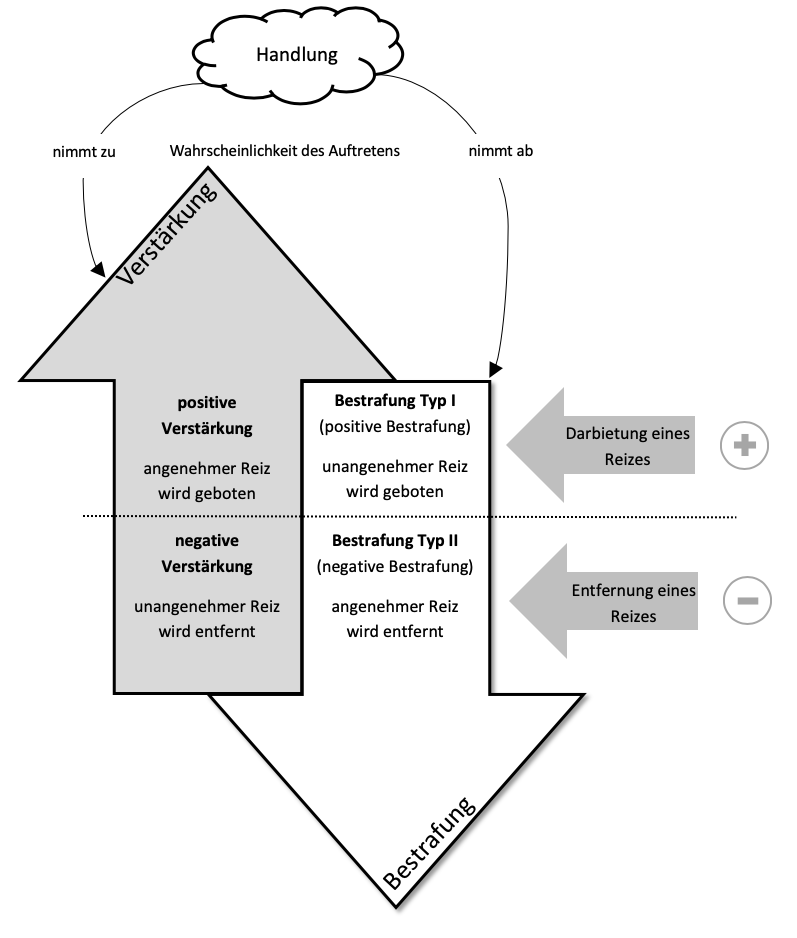
\includegraphics[width=10cm]{Kontingenzschema.png}
	\caption{Kontingenzschemata}
\end{figure}
\end{center}
\begin{itemize}
	\item \textbf{Positive Verstärkung:} Erhöhung der Wahrscheinlichkeit des Auftritts einer Verhaltensweise, wenn die direkte Konsequenz des Verhaltens einer angenehmen Natur ist. 
	\item \textbf{Negative Verstärkung:} Erhöhung der Wahrscheinlichkeit des Auftritts einer Verhaltensweise, wenn das Verhalten eine unangenehme Konsequenz abwehrt.
	\item \textbf{Positive Bestrafung:} Senkung der Wahrscheinlichkeit des Auftritts einer Verhaltensweise, wenn das Verhalten eine unangenehme Konsequenz mit sich zieht.
	\item \textbf{Negative Bestrafung:} Senkung der Wahrscheinlichkeit des Auftritts einer Verhaltensweise, wenn das Verhalten eine angenehme Konsequenz verhindert. 
	\item \textbf{Extinktion:} Wenn eine Verhaltensweise, die zuvor durch Belohnung angelernt wurde auf ein Mal keine positiven Konsequenzen mehr mit sich zieht, wird diese immer seltener auftreten, bis die Verhaltensweise gar nicht mehr auftritt und somit „ausgestorben“ ist. 
\end{itemize}
\subsection{Arten von Verstärkern}
Man unterscheidet grundsätzlich zwischen zwei verschiedenen Arten der Verstärker. Die primären und sekundären Verstärker. 
Ein primärer Verstärker zeichnet sich durch die Eigenschaft aus, dass eine Person mit diesen Reizen geboren wird. Essen, Trinken oder Schmerz sind zum Beispiel primäre Verstärker. 
Sekundäre Verstärker sind Reize, die erlernt werden müssen. Am Anfang sind diese Verstärker neutrale Reize, die nach der Zeit mit Hilfe der primären Verstärker erlernt und gefestigt werden. Geld ist ein gutes Beispiel, da eine Person nach der Geburt nicht wissen kann, dass finanzieller Erfolg eine positive Änderung in Ihrem Leben widerspiegeln kann und erst gelernt werden muss. 
\subsection{Faktoren der Wirksamkeit der Verstärkung und Bestrafung}	
\begin{itemize}
	\item \textbf{Sättigung:} Die Wirksamkeit einer positiven Verstärkung nimmt ab, wenn die Person genug von dieser Belohnung hat. Die Person verliert Interesse.
	\item \textbf{Entzug:} Die Wirksamkeit einer positiven Verstärkung nimmt zu, wenn der Person die Stimulation dieser Belohnung entzogen wird. Wenn ein Verhalten mit Essen belohnt werden würde, hätte ein hungriges Tier eine größere Motivation als ein Tier, dass gerade gegessen hat. 
	\item \textbf{Unmittelbarkeit:} Eine unmittelbare Konsequenz hat einen signifikanteren Lernerfolg als eine verzögerte Konsequenz. 
	\item \textbf{Kontingenz:} Eine Konsequenz sollte immer regelmäßig nach einem Verhalten eintreten. Konsequenzen, die selten Erfolgen, werden langsamer erlernt, was bedeutet, dass das Verhalten seltener auftreten wird. 
	\item \textbf{Volumen:} Die Menge bzw. die Größe einer Belohnung erhöht bzw. senkt meistens die Wirkung der Verstärkung. 
\end{itemize}
%Quellen: 
\subsection{Verstärkungspläne}
Verstärkungspläne sind Methoden, die angewendet werden können, um Verhalten auf eine bestimmte Art zu konditionieren. 
Verstärkungspläne treten sowohl in einer natürlichen Umgebung auf als auch in strukturierten Trainingssituationen auf. 
Die durch B. F. Skinner definierten Verstärkungspläne sind: 
\begin{itemize}
	\item Kontinuierliche Verstärkung
	\item Zeitpläne mit festem Verhältnis
	\item Zeitpläne mit festen Intervallen
	\item Zeitpläne mit variablem Verhältnis
	\item Zeitplänen mit variablen Intervallen
\end{itemize}
\subsection{Kontinuierliche Verstärkung}
Bei jedem erwünschten Verhalten wird verstärkt, die Person lernt schneller aber verlernt dieses Verhalten wiederum auch schneller, wenn die kontinuierliche Verstärkung abnimmt oder beendet wird. 
Eine kontinuierliche Verstärkung kann gut in der initialen Phase einer Konditionierung zur Verwendung kommen, um den Lernerfolg am Anfang stark zu steigern.
Um das Verlernen des Verhaltens vorzubeugen, müssen Verstärkungen nach bestimmten Zeitabständen neu durchgeführt werden. 
%Quellen: https://www.verywellmind.com/what-is-a-fixed-ratio-schedule-2795190 
\subsection{Zeitpläne mit festem Verhältnis}	
Die Verstärkung tritt erst nach einer bestimmten Häufigkeit des Auftretens von erwünschten Verhaltensmustern auf.
Resultiert in häufigem und gleichmäßigem Auftreten von erwünschten Verhaltensmustern. Möglicherweise führt diese Methode zu einem kurzen Stopp der erwarteten Verhaltensweise, nachdem eine Belohnung gegeben wurde. 
Kann sehr gut verwendet werden, um neue Verhaltensmuster zu lernen.
%Quellen: https://www.verywellmind.com/what-is-a-fixed-interval-schedule-2795189
\subsection{Zeitpläne mit festen Intervallen}
Die Verstärkung wird erst nach einer definierten Zeit ausgegeben, wobei das Verhalten bei dieser Methode keine Rolle spielt. 
Resultiert in einer signifikanten Pausierung der erwünschten Verhaltensmuster. Wenn es wieder Zeit für eine neue Verstärkung wird, treten die erwarteten Verhaltensmuster nach und nach immer häufiger auf. 
%Quellen: https://www.verywellmind.com/what-is-a-variable-ratio-schedule-2796012
\subsection{Zeitpläne mit variablem Verhältnis}
		Die Verstärkung erfolgt, wenn ein erwünschtes Verhaltensmuster auftritt. Dabei kann auch definiert werden, dass die Verstärkung nach einer ungefähren Anzahl an Reaktionen erfolgt. Diese Eigenschaften machen diese Methode zu einem bestimmten Grad unvorhersehbar, und steigern die Lernkurve. 
Zeigt erhöhte und gleichmäßige Wahrscheinlichkeit eines Verhaltens. Es tritt eine kurze Verhaltenspause nach der Verstärkung auf. 
%Quellen: https://www.verywellmind.com/variable-interval-schedule-2796011 
\subsection{Zeitplänen mit variablen Intervallen}
Verstärkung erfolgt nach einer zufälligen Zeit in einer vordefinierten Zeitspanne. 
Diese Methode hat eine hohe Resistenz gegen Extinktion. Die Wahrscheinlichkeit einer erwünschten Reaktion ist moderat, aber konsistent und es gibt eine sehr kleine Verhaltenspause nach einer Belohnung. 
\subsection{Nichtkontingente Verstärkung}
Nichtkontingente Verstärkung beschreibt die Abnahme von Verhaltensmustern unabhängig vom Verhalten der Person. Die Nichtkontingente Verstärkung kann verwendet werden, um die Wahrscheinlichkeit eines unerwünschten Verhaltens zu reduzieren, in dem man andere, Verhaltensmuster, die nicht erwünscht sein müssen, aber nicht, nicht erwünscht sind, belohnt und somit das unerwünschte Verhalten abtrainiert, ohne es selbst zu behandeln. 
\subsection{Umsetzung in EMS}
EMS bietet zwei verschiedene Formen der positiven Verstärkung in Form einer materiellen Belohnung mit festem Verhältnis, den Goodies und einer immateriellen Belohnung mit festem Verhältnis, den Leaderboards und eine positive Bestrafung mit festen Intervallen, dem Punkteverfall nach einer bestimmten Zeitspanne der Inaktivität.
Es war ein großes Anliegen in EMS ein sinnvolles und gut durchdachtes Belohnungssystem, dass Motivation ankurbelt, zu implementieren.
Ein funktionierendes Motivationssystem trägt dazu bei, dass Promoter, also die Kartenverkäufer, ihre Leistung immer weiter steigern wollen und somit den Kartenverkauf des Events optimieren. 
Um die Promoter/innen davon abzuhalten ihre Verkaufszahlen nicht zeitgerecht einzutragen, bzw. Sie davon abzuhalten, nach einem bestimmten Verdienst von Punkten nicht weiter Karten zu verkaufen wurde ein Punkteverfall implementiert. Nach einer definierten Zeitspanne von Inaktivität, also einer bestimmten Zeit, in der keine Änderungen im Kartenstand eines/r Promoter/in eingetragen wurde, werden Punkte wieder abgezogen.
Ein/e Promoter/in bekommt nach einer bestimmten Anzahl von Karten Punkte. Diese Punkte werden für jedes Event, an dem der/die Promoter/in teilnimmt gespeichert. 
Promoter/innen können diese Punkte für Goodies, also Belohnungen, die für jedes Event einzeln erstellt werden können, eintauschen. 
Es wird auch für jedes Event eine Rangliste, das Leaderboard, geführt. In diesem Leaderboard werden die zehn verkaufsstärksten Promoter/innen in Riehenfolge mit dem genauen Punktestand aufgeführt. 
\begin{center}
\begin{figure}[h]
	\centering
	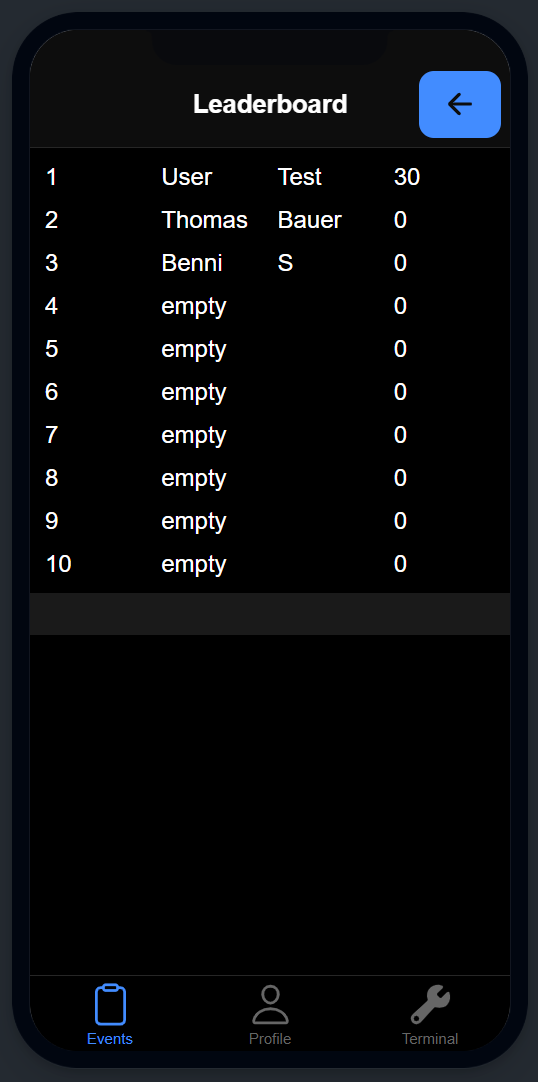
\includegraphics[width=7cm]{Leaderboard.png}
	\caption{Leaderboard eines Events}
\end{figure}
\end{center}
Punkte werden für jede/n Promoter/in auf der Seite des spezifischen Events angezeigt. 
\begin{center}
\begin{figure}[h]
	\centering
	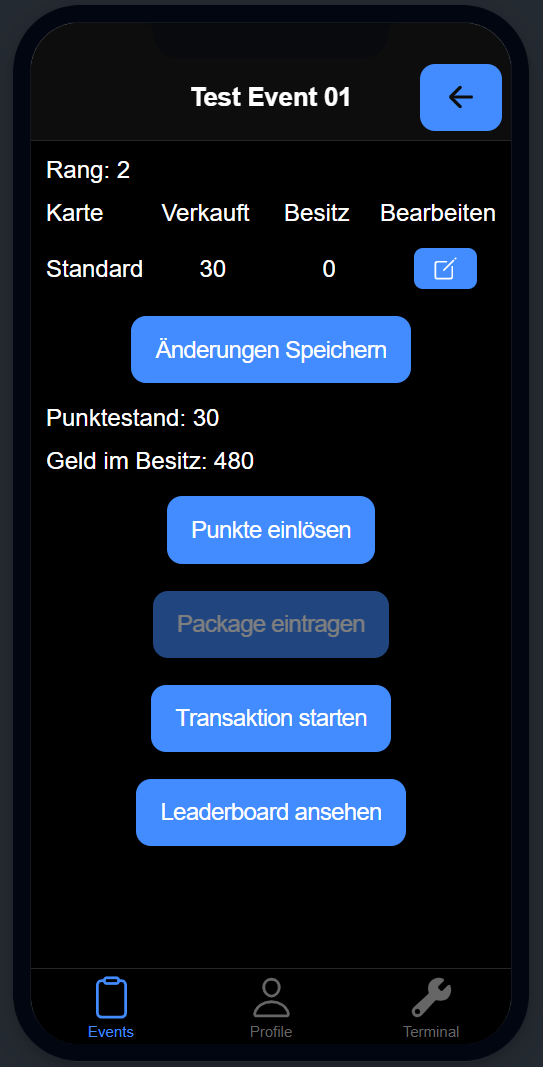
\includegraphics[width=7cm]{Event-Detail.png}
	\caption{Eventdetail eines Events mit angezeigtem Punktestand}
\end{figure}
\end{center}
Promoter/innen können auf den Button „Punkte einlösen“ klicken, um sich Goodies anzeigen zu lassen, für die sie ihre Punkte einlösen können. Goodies werden für jedes Event einzeln definiert und können von Rabatten bis zu Hotelzimmer reichen.
Bei Klick auf „Leaderboard ansehen“ wird der/die Promoter/in auf eine Seite weitergeleitet, die die zehn verkaufsstärksten Promoter anzeigt. 